\section{はじめに}

\begin{frame}{はじめに}
  \begin{itemize}
    \item Beamer のサンプルです
  \end{itemize}
\end{frame}

\section{箇条書き}

\begin{frame}{箇条書き}
  \begin{itemize}
    \item 番号なしの箇条書きです
    \item 番号なしの箇条書きです
    \item 番号なしの箇条書きです
    \item 番号なしの箇条書きです
  \end{itemize}
\end{frame}

\begin{frame}{番号付き箇条書き}
  \begin{enumerate}
    \item 番号付きの箇条書きです
    \item 番号付きの箇条書きです
    \item 番号付きの箇条書きです
  \end{enumerate}
\end{frame}

\begin{frame}{箇条書きのレベル}
  \begin{itemize}
    \item 箇条書きのレベル1です
    \begin{itemize}
      \item 箇条書きのレベル2です
      \begin{itemize}
        \item 箇条書きのレベル3です
      \end{itemize}
      \item 箇条書きのレベル2です
      \item 箇条書きのレベル2です
    \end{itemize}
    \item 箇条書きのレベル1です
  \end{itemize}
\end{frame}


\begin{frame}{箇条書きのレベル}
  \begin{enumerate}
    \item 箇条書きのレベル1です
    \begin{enumerate}
      \item 箇条書きのレベル2です
      \begin{enumerate}
        \item 箇条書きのレベル3です
      \end{enumerate}
      \item 箇条書きのレベル2です
      \item 箇条書きのレベル2です
    \end{enumerate}
    \item 箇条書きのレベル1です
  \end{enumerate}
\end{frame}


\section{ブロック}

\begin{frame}{いくつかのブロック}
  \begin{block}{block}
    \begin{itemize}
      \item block 環境を使ってみます.
    \end{itemize}
  \end{block}
  \begin{alertblock}{alertblock}
    \begin{itemize}
      \item alertblock 環境を使ってみます.
    \end{itemize}
  \end{alertblock}
  \begin{exampleblock}{exampleblock}
    \begin{itemize}
      \item exampleblock 環境を使ってみます.
    \end{itemize}
  \end{exampleblock}
\end{frame}


\begin{frame}{見出しのないブロック}
  \begin{block}{}
    \begin{itemize}
      \item block 環境を使ってみます.
    \end{itemize}
  \end{block}
  \begin{alertblock}{}
    \begin{itemize}
      \item alertblock 環境を使ってみます.
    \end{itemize}
  \end{alertblock}
  \begin{exampleblock}{}
    \begin{itemize}
      \item exampleblock 環境を使ってみます.
    \end{itemize}
  \end{exampleblock}
\end{frame}

\begin{frame}{定理と証明(thm)}
  \begin{thm}
    \begin{itemize}
      \item 定理(thm)環境を使ってみます.
    \end{itemize}
  \end{thm}
  \begin{proof}
    証明はproof環境です.証明はproof環境です.証明はproof環境です.証明はproof環境です.証明はproof環境です.証明はproof環境です.自動的に証明おわりの記号が右端に出力されます.
  \end{proof}
\end{frame}

\begin{frame}{命題 (proposition)}
  \begin{proposition}
    \begin{itemize}
      \item 命題(proposition)環境を使ってみます.
      \item 命題(proposition)環境を使ってみます.
    \end{itemize}
  \end{proposition}
\end{frame}

\begin{frame}{例題 (exam)}
  \begin{exam}
    \begin{itemize}
      \item 例題(exam)環境を使ってみます.
      \item 通常のブロック要素と色が異なることに注意してください.
    \end{itemize}
  \end{exam}
\end{frame}

\begin{frame}{注 (remark)}
  \begin{remark}
    \begin{itemize}
      \item 注(remark)環境を使ってみます.
      \item 通常のブロック要素と色が異なることに注意してください.
    \end{itemize}
  \end{remark}
\end{frame}

\begin{frame}{問題 (question)}
  \begin{question}
    \begin{itemize}
      \item 問題(question)環境を使ってみます.
      \item 通常のブロック要素と色が異なることに注意してください.
    \end{itemize}
  \end{question}
\end{frame}

\begin{frame}{問題 (prob)}
  \begin{prob}
    \begin{itemize}
      \item 問題(prob)環境を使ってみます.
      \item 通常のブロック要素と色が異なることに注意してください.
    \end{itemize}
  \end{prob}
\end{frame}

\section{数式,図,表}

\begin{frame}{数式}
  \begin{itemize}
    \item 数式$F(t)$は\LaTeX~の書き方がほぼ使えるはず
    \begin{equation}
      F(t) = \int_{0}^{t}f(x)dx
    \end{equation}
    \item 数式番号が不要であれば
    \begin{equation*}
      F(s) = \int_{0}^{\infty}f(t)e^{-st}dt
    \end{equation*}
    \item 複数行の数式ももちろん可能
    \begin{eqnarray*}
      F(t) &=& \int_{0}^{t}f(x)dx \\
      &=& 1 - e^{-\lambda t}
    \end{eqnarray*}
  \end{itemize}
\end{frame}

\begin{frame}{画像(PDF形式)の読み込み}
  \begin{figure}
    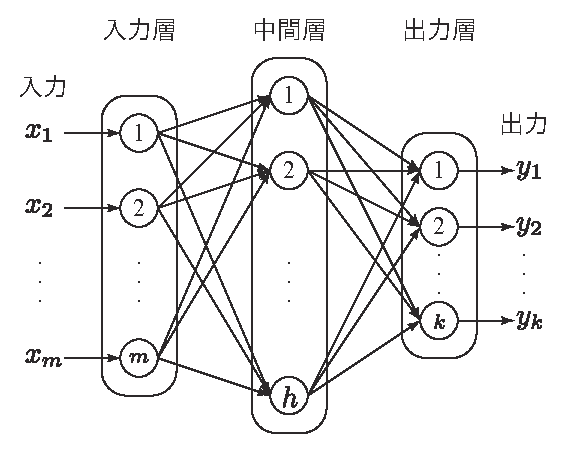
\includegraphics[width=70mm]{figs/nn.pdf}
  \end{figure}
\end{frame}

\begin{frame}{画像(PNG形式)の読み込み}
  \begin{figure}
    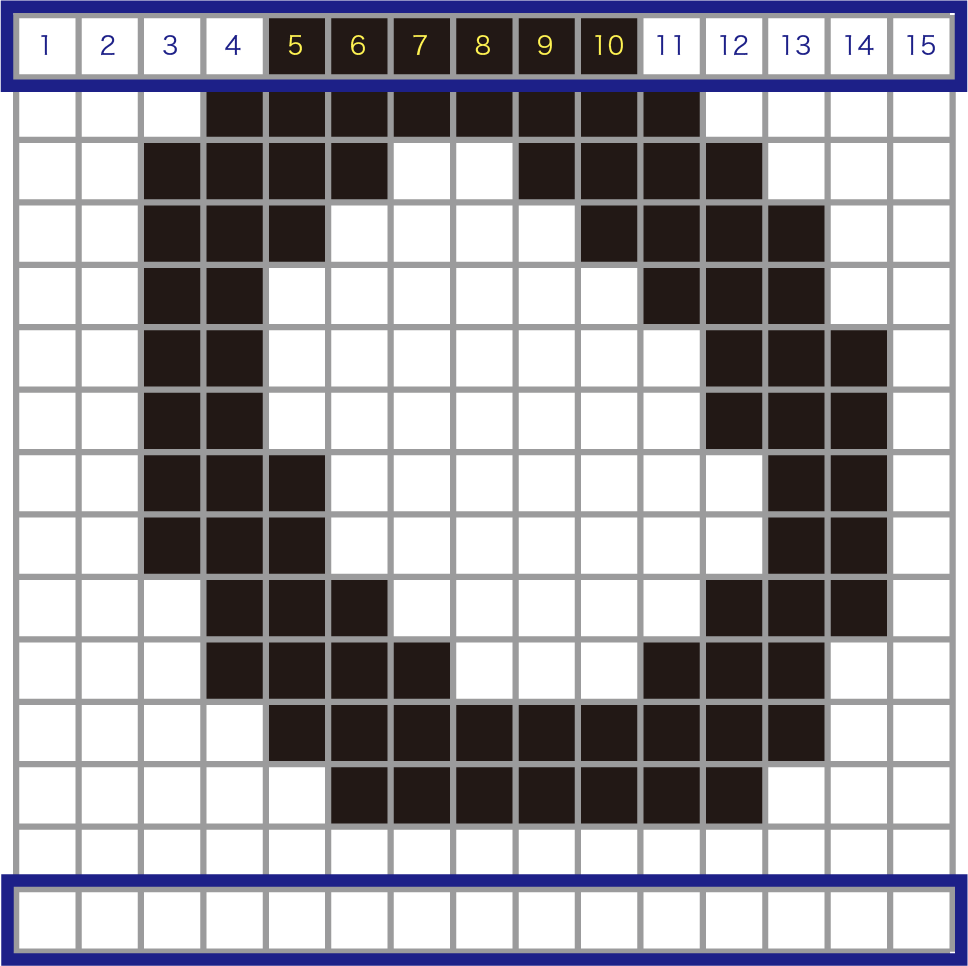
\includegraphics[width=60mm]{figs/tegaki-0-01-rgba.png}
  \end{figure}
\end{frame}


\begin{frame}{表}
  \begin{center}
    \begin{tabular}{clr}
      \Hline
      \multicolumn{1}{c}{中央揃え} &
      \multicolumn{1}{c}{左揃え} &
      \multicolumn{1}{c}{右揃え} \\ \Hline
      2018 & AAAAA & 22222 \\ \hline
      2019 & AA & 2222 \\ \hline
      2020 & AAAAA & 22 \\ \hline
      2021 & AAAAAAAAAA & 222 \\ \hline
      2022 & A & 2 \\ \Hline
    \end{tabular}
  \end{center}
  なお,横線は \texttt{\textbackslash hline} ですが,太線 \texttt{\textbackslash Hline} も定義しています.
\end{frame}

\section{フォント,色の指定,その他スタイルの指定とアニメーション}

\subsection{フォントと色}

\begin{frame}{フォントや色を指定する}
  \begin{itemize}
    \item 通常のフォントはゴシック(Gothic 01234)です.
    \item {\bgoth 太字のゴシック体です.}
    \item {\minc かな文字を明朝体(minc 01234)に変更できます.}
    \item {\rm Roman}, \textit{textit}, \textsl{textsl}, \textsf{textsf}, \textrm{textrm}, \texttt{texttt}
    \item 標準はグレーです.{\color{black}色(black)を黒に変更します.}
    \item {\color{blue}色(blue)を変更します.}
    \item {\color{magenta}\bgoth 色(magenta)と書体を}{\color{red}\bgoth (red)変更します.}
    \item {\color{beamer@kgured}\bgoth beamer@kgured} と {\color{beamer@kgublue}\bgoth beamer@kgublue} を定義しています.{\color{beamer@kgublue}\bgoth beamer@kgublueはヘッダロゴや見出しと同色です}
  \end{itemize}
\end{frame}

\begin{frame}{フォントサイズを変更する}
  \begin{itemize}
    \item {\tiny tiny フォントサイズです}
    \item {\scriptsize scriptsize フォントサイズです}
    \item {\footnotesize footnotesize フォントサイズです}
    \item {\small small フォントサイズです}
    \item {\normalsize normalsize (標準)フォントサイズです}
    \item {\large large フォントサイズです}
    \item {\Large Large フォントサイズです}
    \item {\LARGE LARGE フォントサイズです}
    \item {\huge huge フォントサイズです}
    \item {\Huge Huge フォントサイズです}
  \end{itemize}
\end{frame}

\subsection{背景の変更}
{
\usebackgroundtemplate{
\includegraphics[width=\paperwidth]{kgu-bg169ruled.pdf}}
\begin{frame}{背景を変更}
  \begin{itemize}
    \item このページだけ背景を変更します
  \end{itemize}
\end{frame}
}

\subsection{配置の変更}

\begin{frame}[t]{箇条書きの配置をページの上部に}
  \begin{itemize}
    \item $[\mbox{t}]$ オプションを指定すると箇条書きが上部に配置される
    \item $[\mbox{t}]$ オプションを指定すると箇条書きが上部に配置される
  \end{itemize}
\end{frame}

\subsection{段組}

\begin{frame}{2段組み}
  \begin{columns}
    \begin{column}{0.5\textwidth}
      \begin{itemize}
        \item 2段組みです.2段組みです.2段組みです.2段組みです.2段組みです.2段組みです.2段組みです.2段組みです.2段組みです.2段組みです.2段組みです.2段組みです.2段組みです.
      \end{itemize}
    \end{column}
    \begin{column}{0.5\textwidth}
      \begin{itemize}
        \item 2段組みです.2段組みです.2段組みです.2段組みです.2段組みです.2段組みです.2段組みです.2段組みです.2段組みです.2段組みです.2段組みです.2段組みです.2段組みです.2段組みです.2段組みです.2段組みです.2段組みです.2段組みです.
      \end{itemize}
    \end{column}
  \end{columns}
\end{frame}

\begin{frame}{2段組み(比率の変更と上部配置)}
  \begin{columns}[t]
    \begin{column}{0.3\textwidth}
      \begin{itemize}
        \item 2段組みです.2段組みです.2段組みです.2段組みです.2段組みです.2段組みです.2段組みです.2段組みです.2段組みです.2段組みです.2段組みです.2段組みです.2段組みです.
      \end{itemize}
    \end{column}
    \begin{column}{0.7\textwidth}
      \begin{itemize}
        \item 2段組みです.2段組みです.2段組みです.2段組みです.2段組みです.2段組みです.2段組みです.2段組みです.2段組みです.2段組みです.2段組みです.2段組みです.2段組みです.2段組みです.2段組みです.2段組みです.2段組みです.2段組みです.
      \end{itemize}
    \end{column}
  \end{columns}
\end{frame}

\subsection{アニメーション}

\begin{frame}{アニメーション}
  \begin{itemize}
    \item アニメーションを使います.
    \pause
    \item 2つ目の項目です.
    \item ページ番号は変化しないことに注意してください.
    \pause
    \item 3つ目の項目です.
  \end{itemize}
\end{frame}

\begin{frame}{アニメーション(順序の指定)}
  \begin{itemize}
    \item<1-> アニメーションを使います.
    \item<3-> 2つ目の項目です.
    \item<2-> 3つ目の項目です.
  \end{itemize}
\end{frame}

\begin{frame}{表のアニメーション(1)}
  \begin{itemize}
    \item \texttt{\textbackslash pause}を使ったアニメーション
  \end{itemize}
  \begin{center}
    \begin{tabular}
      {clr}
      \Hline
      \multicolumn{1}{c}{中央揃え} &
      \multicolumn{1}{c}{左揃え} &
      \multicolumn{1}{c}{右揃え} \\ \Hline
      2018 & AAAAAAAA & 22222222 \\ \hline \pause
      2019 & AAAAAA & 222222 \\ \hline
      2020 & AAAA & 2222 \\ \hline \pause
      2021 & AA & 22 \\ \hline
      2022 & A & 2 \\ \Hline
    \end{tabular}
  \end{center}
\end{frame}

\begin{frame}{表のアニメーション(2)}
  \begin{itemize}
    \item 順序のコントロール
  \end{itemize}
  \begin{center}
    \begin{tabular}
      {clr}
      \Hline
      \multicolumn{1}{c}{中央揃え} &
      \multicolumn{1}{c}{左揃え} &
      \multicolumn{1}{c}{右揃え} \\ \Hline
      \onslide<4->2018 & AAAAAAAA & 22222222 \onslide<1-> \\ \hline
      \onslide<3->2019 & AAAAAA & 222222 \onslide<1-> \\ \hline
      \onslide<2->2020 & AAAA & 2222 \onslide<1-> \\ \hline
      2021 & AA & 22 \\ \hline
      2022 & A & 2 \\ \Hline
    \end{tabular}
  \end{center}
\end{frame}

\begin{frame}{表のアニメーション(3)}
  \begin{itemize}
    \item 列のアニメーション(強引な手法ですが)
  \end{itemize}
  \begin{center}
    \begin{tabular}
      {clr}
      \Hline
      \multicolumn{1}{c}{中央揃え} &
      \multicolumn{1}{c}{左揃え} &
      \multicolumn{1}{c}{右揃え} \\ \Hline
      2018 & \onslide<2->AAAAAAAA & \onslide<3->22222222 \onslide<1->\\ \hline
      2019 & \onslide<2->AAAAAA & \onslide<3->222222 \onslide<1->\\ \hline
      2020 & \onslide<2->AAAA & \onslide<3->2222 \onslide<1->\\ \hline
      2021 & \onslide<2->AA & \onslide<3->22 \onslide<1->\\ \hline
      2022 & \onslide<2->A & \onslide<3->2 \onslide<1->\\ \Hline
    \end{tabular}
  \end{center}
\end{frame}

\begin{frame}{おわり}
  \begin{itemize}
    \item 以上Beamerのサンプルでした
  \end{itemize}
\end{frame}
